\documentclass[border=10pt]{standalone}
\usepackage{tikz}
\usepackage{amsmath}
\usepackage{amssymb}
\usetikzlibrary{arrows.meta, shadows, positioning}

% Macro used in your equation
\newcommand{\vect}[1]{\boldsymbol{#1}}

% Color palette
\definecolor{accent}{HTML}{1F4E79}
\definecolor{softaccent}{HTML}{EAF2F8}
\definecolor{softgray}{HTML}{F6F7F9}

\begin{document}
	
	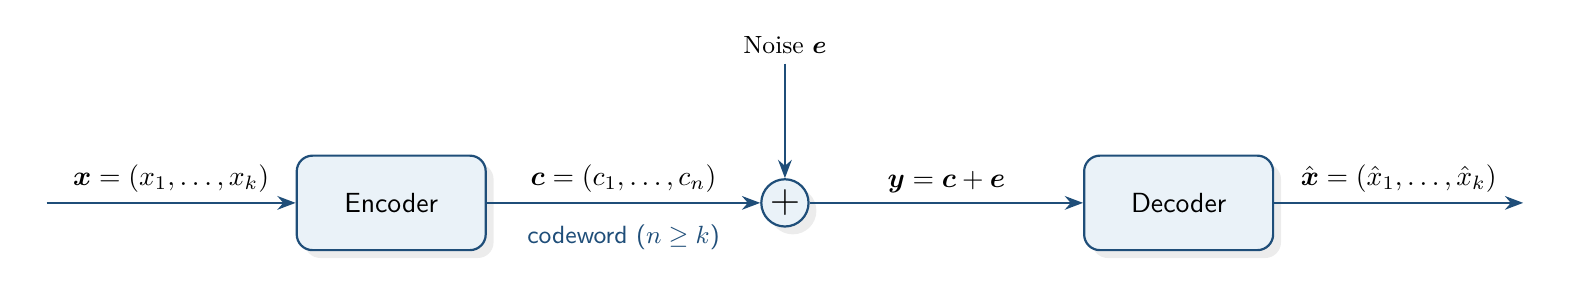
\begin{tikzpicture}[
		>=Stealth,
		block/.style={
			draw=accent, thick, fill=softaccent, rounded corners=2mm,
			minimum width=2.4cm, minimum height=1.2cm, align=center,
			font=\sffamily, drop shadow={opacity=0.15, shadow xshift=1mm, shadow yshift=-1mm}
		},
		adder/.style={
			circle, draw=accent, thick, fill=softaccent,
			minimum size=6mm, inner sep=0pt, align=center, font=\Large,
			drop shadow={opacity=0.15, shadow xshift=1mm, shadow yshift=-1mm}
		},
		arrow/.style={->, thick, accent},
		mathlabel/.style={font=\normalsize, text=black},
		sublabel/.style={font=\small\sffamily, text=accent}
		]
		
		% Invisible nodes to act as the start and end points of the signals
		\node (start) at (0,0) {};
		\node (end)   at (19,0) {};
		
		% Main operational blocks
		\node[block] (enc) at (4.5,0) {Encoder};
		\node[adder] (add) at (9.5,0) {$+$};
		\node[block] (dec) at (14.5,0) {Decoder};
		
		% Noise entry point
		\node (noise) at (9.5, 2) {\small Noise $\vect{e}$};
		
		% --- Signal Paths & Labels ---
		
		% Source to Encoder
		\draw[arrow] (start) -- 
		node[above, mathlabel] {$\vect{x}=(x_1,\dots,x_k)$} 
		(enc);
		
		% Encoder to Channel (Adder)
		% We use a standard label below the arrow to replace the underbrace in the equation
		\draw[arrow] (enc) -- 
		node[above, mathlabel] {$\vect{c}=(c_1,\dots,c_n)$} 
		node[below=1.5mm, sublabel] {codeword ($n \geq k$)} 
		(add);
		
		% Noise entering the Channel
		\draw[arrow] (noise) -- (add);
		
		% Channel to Decoder
		\draw[arrow] (add) -- 
		node[above, mathlabel] {$\vect{y}=\vect{c}+\vect{e}$} 
		(dec);
		
		% Decoder to Destination
		\draw[arrow] (dec) -- 
		node[above, mathlabel] {$\hat{\vect{x}}=(\hat x_1,\dots,\hat x_k)$} 
		(end);
		
	\end{tikzpicture}
	
\end{document}